 \chapter{The Multiscale Frangi Filter and other Variations} \label{ch:multifrangi}
    
    
    	\begin{figure}[p] \centering % scale sweep, large plate
    	\subfloat{        \label{fig:scalesweep-1p}\includegraphics[width=\linewidth]{{{scalesweep_stitch_BN2315363_plate}}}
    	} \\[-0.5cm]
    	\subfloat{        \label{fig:scalesweep-1i}\includegraphics[width=\linewidth]{{{scalesweep_stitch_BN2315363_inset}}}
    	} \\[-0.5cm]
    	\subfloat{        
    		\label{fig:scalesweep-1c}\includegraphics[width=.75\linewidth]{{{scalesweep_colorbar}}}
    	} \\[12pt]
    	% should i use the real sample names? or obfuscate?
    	\caption{Example scalewise Frangi output (plate and inset) (example 1)}
    	\label{fig:scalesweep-1}
    \end{figure}
    
    \begin{figure}[p] \centering % scale sweep, small plate
    	\subfloat{        \label{fig:scalesweep-2p}\includegraphics[width=\linewidth]{{{scalesweep_stitch_BN5280796_plate}}}
    	} \\[-0.5cm]
    	\subfloat{        \label{fig:scalesweep-2i}\includegraphics[width=\linewidth]{{{scalesweep_stitch_BN5280796_inset}}}
    	} \\[-0.5cm]
    	\subfloat{        
    		\label{fig:scalesweep-2c}\includegraphics[width=.75\linewidth]{{{scalesweep_colorbar}}}
    	} \\[12pt]
    	\caption{Example scalewise Frangi output (plate and inset) (example 2)}
    	\label{fig:scalesweep-2}
    \end{figure}

    With the notion of scale space established, we return to the task of computing the Frangi filter for discrete images. We repeat our final definition of the Frangi filter here, now encoding an explicit choice of scale, $\sigma$.
    
    \begin{gather} \label{eq:Vsigma}
    \Vsigma(x_0,y_0) = \begin{cases}
    0 & \text{if} \quad \lambda_2 > 0 \\
    a_\gamma \exp\left(\frac{-\Am^2}{2\beta^2}\right)
    \left(1 - \exp\left(\frac{-\Sm^2}{2(\gamma \Smax)^2}\right)\right) & \text{otherwise}
    \end{cases} \\
    \shortintertext{where}
    %\begin{equation} \label{frangi-def-anisotropy-structureness-v1}
    \Am := \abs*{\frac{\lambda_1}{\lambda_2}}
    \;,\;
    \Sm := \sqrt{\lambda_1^2 + \lambda_2^2}
    \;\textrm{and}\;
    a_\gamma = \left(1-\exp\left(\frac{-1}{2\gamma^2}\right)\right)^{-1} \notag\\
    %\end{equation}
    \end{gather}
    and $\abs*{\lambda_1} \le \abs*{\lambda_2}$
    are eigenvalues of the Hessian matrix at point $(x_0, y_0)$ at scale $\sigma.$

    A central point of importance here is that certain ridgelike structures will be more prominent at different scales. \cref{fig:scalesweep-1} and \cref{fig:scalesweep-2} demonstrate this effect for two different placental samples. Here, a Frangi filter is applied to the sample at eight different scales ranging from small to large. The vesselness response is greater at smaller scales for smaller width vessels and smaller for larger width vessels. When the scale is large, the reverse is true: response to small vessels is nonexistent, and larger scales are prominent.  A full treatment of applying the Frangi filter to these samples begins in \cref{ch:research-protocol}.
    
    \section{The Multiscale Frangi Filter}
    Since our eventual goal is a complete extraction of the vasuclar network, a multiscale approach is the natural one. Considering the dependence of the Frangi filter's response on choice of scale as demonstrated in \cref{ch:unifrangi}, we wish to probe at multiple scales
   regions that would receive a high vesselness score at any range and somehow merge the result.
   
    Frangi (\citeyear{frangi-paper}) approached this problem by simply taking the maximum vesselness measure over all scales. Thus the multiscale Frangi vesselness score at the pixel $(x_0, y_0$) would be 
    
    \begin{equation} \label{eq:Vmax}
    \Vmax(x_0, y_0) :=
    	\underset{\sigma \in \Sigma}{\max}\left\{  \Vsigma (x_0, y_0) \right\}
    \end{equation}
    
    where $\Sigma := \left\{ \sigma_0, \sigma_1 , \cdots, \sigma_n \right\}$ is
    the set of $n$ scales at which to probe, and \Vsigma is the Frangi vesselness measure at scale $\sigma$ for the pixel $(x_0,y_0)$, as given in \cref{eq:Vsigma}.
    Occasionally it will be useful to refer to the scale at which $\Vmax$ occurs for a 
    particular pixel, so we analogously define
    
    \begin{equation} \label{eq:Vargmax}
    \Vargmax(x_0, y_0) := \underset{\sigma \in \Sigma}{\arg\max}\left\{  \Vsigma (x_0, y_0) \right\}
    \end{equation}
The set of scales $\Sigma$ should be chosen to be representative enough of all scales where meaningful content is expected to be found. Unfortunately this appropriate range of scales may not be known \textit{a priori}. We will address this issue in \cref{ch:segmentation}.

Finally, we may also wish to deal with the unmerged vesselness measures as a whole, i.e. without taking a maximum at all. In this case, we will refer to $\VSigma$, the 3D matrix of shape
$n \times (M\times N)$, where $M$ and $N$ are the dimensions of the image matrix $\img$
as in \cref{def:image_as_pixel_matrix}.
	\begin{equation} \label{eq:VSigma}
	\VSigma(x_0,y_0 ; \sigma) := \Vsigma(x_0,y_0)
\end{equation}

    
    After the maximization in \cref{eq:Vmax}, we are left with a matrix with as many pixels as the original image, all with a vesselness measure between $0$ and $1$ for each pixel in the image.
         
    At this point, Frangi (\citeyear{frangi-paper}) refrained from explicitly interpreting the score assigned by \cref{eq:Vmax}; that is--whether a particular pixel $(x_0,y_0)$ in the image definitely respresents a vessel or not based on its Frangi score. Instead, he cautioned that the result should not be used as a segmentation method alone; moreover, the width of the vasculature cannot be determined rigorously from the Frangi filter, as discussed in \cref{ch:unifrangi}. 
   
    Nonetheless, we wish to demonstrate the usefulness of the Frangi filter within our image domain towards segmentation. We should at least expect that a well-tuned Frangi filter on an appropriately registered and denoised sample should assign its highest scores to vessel pixels. We can select these strong Frangi responses and use them as seeds for some subsequent algorithm. We will discuss methods of harnessing the Frangi result to the task of segmentation in \cref{ch:segmentation}.
    
    We briefly discuss two variations on the Frangi filter which will prove useful in turn.



\section{The Signed Frangi Filter} \label{sec:signed-frangi-filter}
We finally introduce the novel (yet straightforward) notion of the signed Frangi filter. As will be shown in \cref{ch:segmentation}, we can befefit from simultaneously calculate for a dark background and a light background. Since the Frangi filter normally throws away any response where $\lambda_2 < 0$ (if dark curvilinear features are targeted) or $\lambda_2 >0$ (if light curvilinear features are targeted), we lose no computation time at all (although we must store more results). After computing the multiscale result, we can easily separate these into a positive and a negative strain, which we will denote
$\Vmax^{(+)}$ and $\Vmax^{(-)}$. Our $\Vmax^{(+)}$ is the same as our $\Vmax$ before, and $\Vmax^{(-)}$ is the same result as if we had taken the Frangi filter while only looking for the opposite type (light/dark) curvilinear feature, i.e. by changing the piecewise case of \cref{eq:frangi-vesselness-measure} to $\lambda_2 > 0$. Plotting $\Vmax$ over a scale of $[-1,1]$ demonstrates an interesting effect, as shown in \cref{fig:signsweep-2}. Whereas the Frangi filter generally is not reliable in terms of accurately predicting widths of trough-like (or ridge-like) curvilinear features, we \textit{can} get a sense of the width of the vessel in our particular application by simulataneously considering $\Vmaxpos$ and $\Vmaxneg$. We will develop a method of utilizing this observation in \cref{ch:segmentation}.


All that remains to describe mathematically is how to actually calculate the derivatives of our images and deal with the ultimately discrete nature of our samples.

\section{Weingarten-based Frangi Filter} \label{sec:wein-frangi}

As a final note, even though the Frangi filter uses the eigenvalues of the Hessian matrix as approximations to principal curvatures, we could in fact calculate the eigenvalues of the Weingarten map instead, as given in \cref{weinmatexactgraph}. Indeed, our development of the Frangi filter in \cref{ch:unifrangi} would proceed identically with $\lambda_2$ and $\lambda_1$ being the \textit{true} principal curvatures of the surface. In the case of identifying bright curvilinear structures, we would still like zero filter response when $\lambda_2 > 0$, as this would imply that the surface has positive curvature at that point, indicating a possible valley. Similarly, if we are seeking dark curvilinear structures, we would want to exclude points where $\lambda_2 < 0$, as dark curvilinear structures should not have negative maximum curvatures. Although we retain our focus on the more classical Hessian-based Frangi filter for the remainder of our efforts, we do offer one visual comparison between $\Vmax$ of a Hessian-based Frangi filter and  $\Vmax$ of a Weingarten-based Frangi filter in \cref{fig:compare-wein-hess-Vmax}.
Unfortunately, time did not permit further investivation the Weingarten-based Frangi filter within the scope of this project, but such an effort seems to be a very promising future direction of research.

\begin{figure}[t]\centering
  \subfloat[Raw Sample]{
    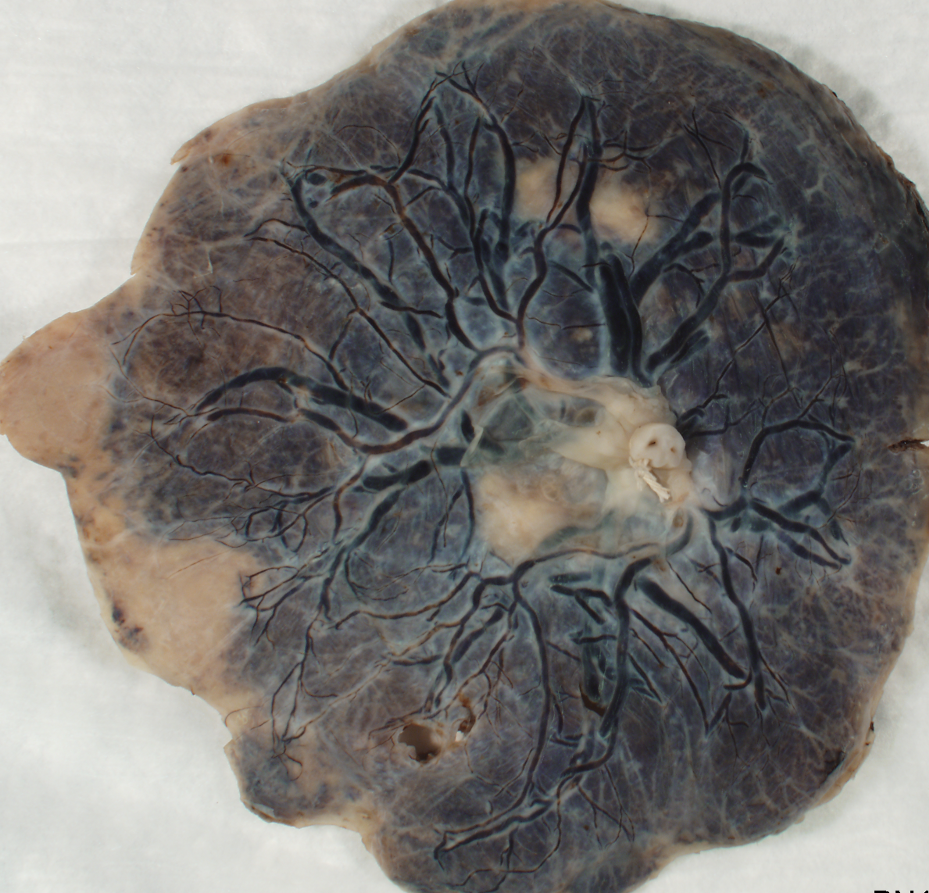
\includegraphics[width=0.32\textwidth]{BN4384182-raw-weindemo}
  }
  \subfloat[$\mathcal{V}_{\max}$ (Hessian-based)]{
    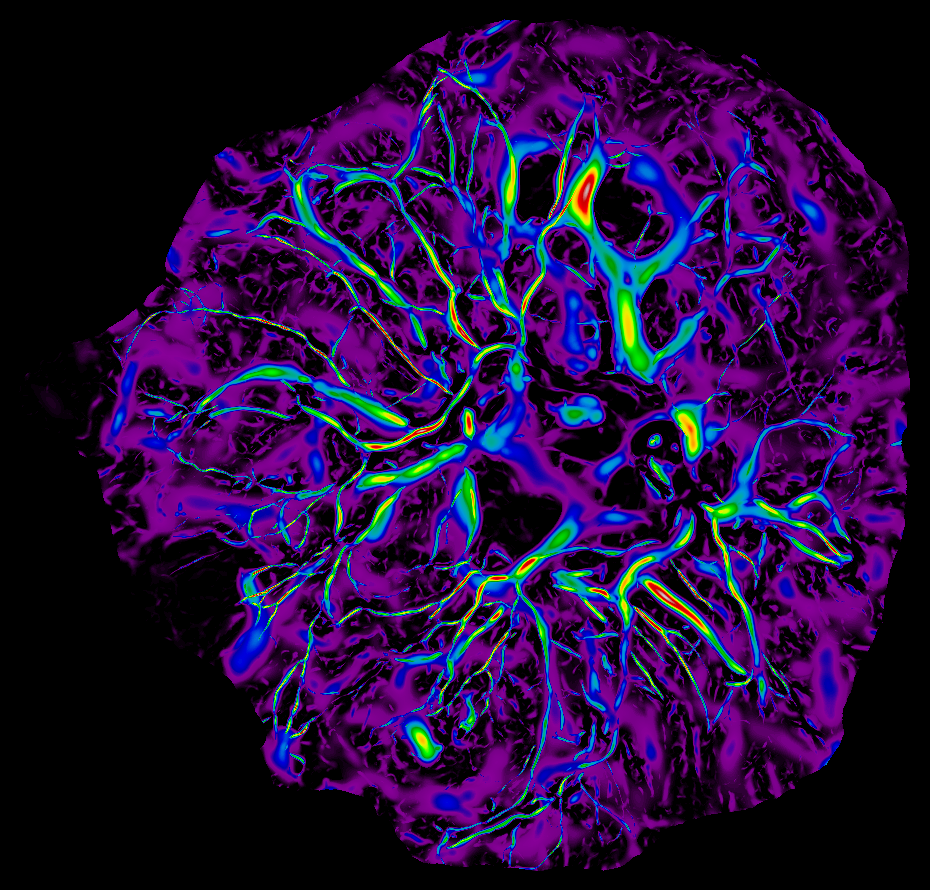
\includegraphics[width=0.32\textwidth]{BN4384182-Vmax-weindemo}
  }
  \subfloat[$\mathcal{V}_{\max}$ (Weingarten-based)]{
    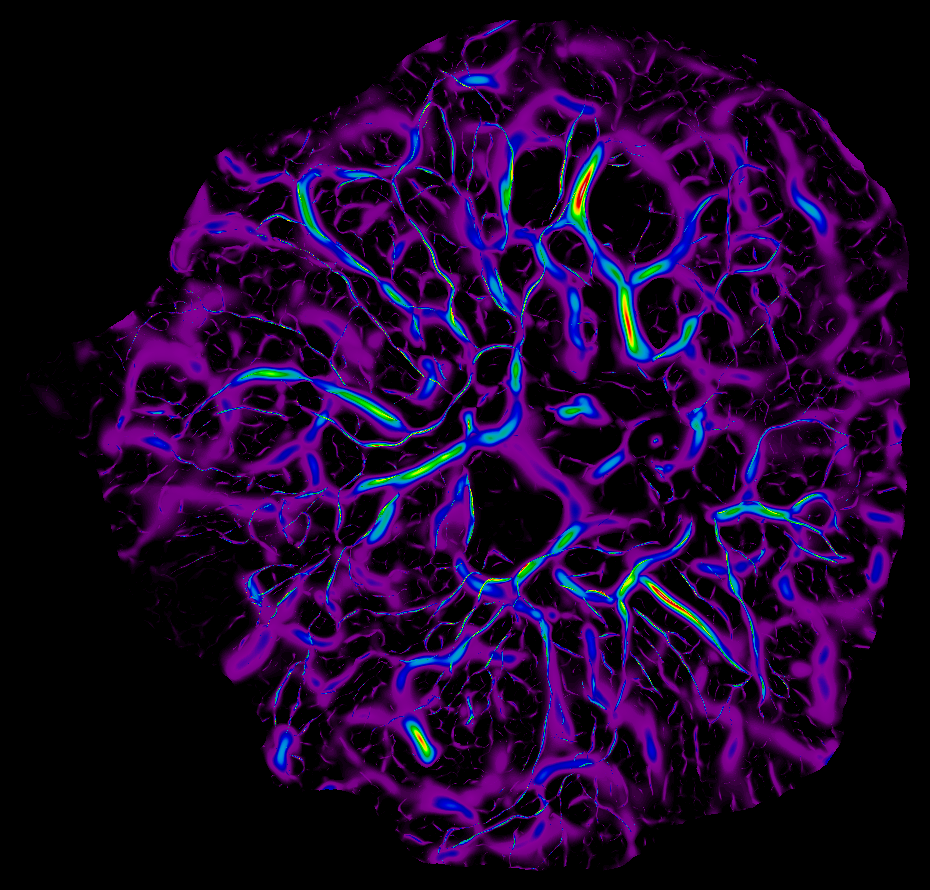
\includegraphics[width=0.32\textwidth]{BN4384182-Wmax-weindemo}
  }
  \\[12pt]
\caption{Comparing Hessian-based and Weingarten-based Frangi filter}
\label{fig:compare-wein-hess-Vmax}
\end{figure}

